\documentclass[a4paper]{scrartcl}
\usepackage{amsmath,amssymb,fvsw,ulem,color}
\usepackage{gmeometric}
\usepackage{lscape}

\newtheorem{ex}{Exercise}
\newenvironment{exercise}[1]%
   {\def\tmp{}%
    \def\points{#1}%
    \ifx\points\tmp
      \begin{ex}
    \else
      \def\tmp{1}%
    \begin{ex}[#1 point\ifx\points\tmp\else s\fi]
    \fi
    \normalfont
   }%
   {\end{ex}%
   }

\usepackage{enumerate}
\newenvironment{subexercises}%
   {\begin{enumerate}[(a)]}%
   {\end{enumerate}}

\renewcommand\paragraph[1]{\medskip\par\noindent\textit{#1}}

\begin{document}
\title{Formal Verification of Software~-- Exercises}
\date{May 2012}
\author{First Author\and Second Author\and Third Author}
\maketitle

\begin{exercise}{1}\label{ex:syntax}
  Show that the \TPL\ program given in exercise~\ref{ex:ifabort}
  is syntactically correct.
\end{exercise}

\subsection{solution}
\textbf{Proof}: Reduction from \textsc{Halting} problem to \textsc{%
Neg-Assignment}.

\noindent Let $(\Pi ,I)$ be an arbitrary instance of \textsc{Halting}, i.e. $\Pi $ \
is a program that takes an input I. Based on this, we have to construct an
instance $(\Pi ^{\prime },I^{\prime },k)$ for \textsc{Neg-Assignment} by
setting $I^{\prime }=I$ and setting initially $k\geq 0$. Then $\Pi ^{\prime
} $ is defined as follows:

%TCIMACRO{%
%\TeXButton{Procedure}{\begin{center}
%\fbox{
%\begin{minipage}[c]{.9\linewidth}
%\small
%boolean $\Pi'$(String $I$) $\{$\\
%   int $k := 0$;\\
%   call $\Pi(I)$;\\
%   $k := -1$;\\
%   return true;\\
%$\}$\\
%
%\end{minipage}
%}
%\end{center}}}%
%BeginExpansion
\begin{center}
\fbox{
\begin{minipage}[c]{.9\linewidth}
\small
boolean $\Pi'$(String $I$) $\{$\\
   int $k := 0$;\\
   call $\Pi(I)$;\\
   $k := -1$;\\
   return true;\\
$\}$\\

\end{minipage}
}
\end{center}%
%EndExpansion

\noindent Let $x=(\Pi ,I)$ be an instance of \textsc{Halting} and $R(x)=(\Pi ^{\prime
},I^{\prime },k)$ the resulting instance from the reduction. Then, we have
to show that $x$ is reducible to $R(x)$ by following equivalence relation:%
\begin{eqnarray*}
&&(\Pi ,I)\text{ is a positive instance of \textsc{Halting}}%
\quad\Leftrightarrow\quad (\Pi ^{\prime },I^{\prime },k)\text{ is apositive
instance} \\
&&\text{of the procedure \textsc{Neg-Assignment}.}
\end{eqnarray*}

(i.e. $\Pi $ halts on $I$ and assigns to $k$ a negative integer value$\quad
\Leftrightarrow\quad \Pi^{\prime }$ returns \textit{true}.)

$\Rightarrow :$ Suppose that $\left( \Pi ,I\right) $ is a positive instance
of \textsc{Halting}, i.e. $\Pi $ terminates on $I$.

\noindent Then by construction of $(\Pi ^{\prime },I^{\prime },k)$, the call of $\Pi
(I^{\prime })$ in program $\Pi ^{\prime }$ terminates since $I^{\prime }=I$.
Hence, $\Pi ^{\prime }$ halts on input $I^{\prime }$, assignes $k:=-1$ and
returns \textit{true} respectively.

\noindent Thus, $(\Pi ^{\prime },I^{\prime },k)$ is a positive instance of \textsc{%
Neg-Assignment}.

\bigskip

$\Leftarrow :$ Suppose that $\left( \Pi ^{\prime },I^{\prime },k\right) $ is
a positive instance of \textsc{Neg-Assignment}, i.e. $\Pi ^{\prime }$
returns \textit{true} after assigning a negative value to $k$. Since $\Pi
^{\prime }$ involves the call of $\Pi (I^{\prime })$ with $I^{\prime }=I$, $%
\Pi $ terminates on $I$ and $k$ will be set to $-1$. Hence, $(\Pi ,I)$ is a
positive instance of \textsc{Halting}.

\bigskip


\begin{exercise}{1}
  Let $\sigma$ be a state satisfying $\sigma(x)=\sigma(y)=1$, and let
  $p$ be the program given in exercise~\ref{ex:ifabort}.
  Compute $\M p\sigma$, using
  \begin{subexercises}
    \item the structural operational semantics
    \item the natural semantics
  \end{subexercises}
  of \TPL.
\end{exercise}

\solution{
	Implication graph:\medskip 
	\begin{figure}[ht]
	\centering
	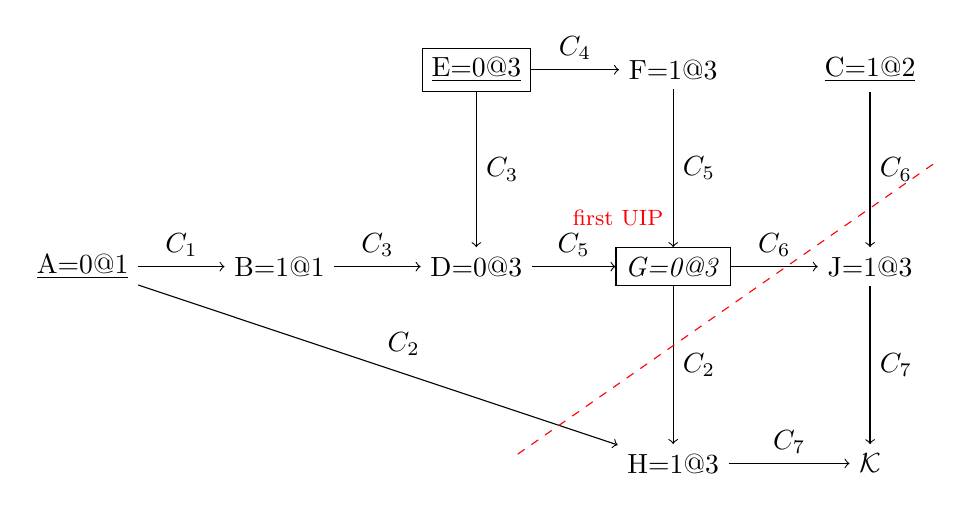
\begin{tikzpicture}[node distance=2.5cm,auto]
	\node (A) {\underline{A=0@1}};
	\node (B) [right of=A] {B=1@1};
	\node (D) [right of=B] {D=0@3};
	%\color{red}
	\node (G) [right of=D, rectangle, draw=black] {\textit{G=0@3}};
	%\color{black}
	\node (H) [below of=G] {H=1@3};
	\node (K) [right of=H] {$\mathcal K$};
	\node (E) [above of=D, rectangle, draw=black] {\underline{E=0@3}};
	\node (F) [right of=E] {F=1@3};
	\node (J) [right of=G] {J=1@3};
	\node (C) [above of=J] {\underline{C=1@2}};
	\path[->] (G) edge node {$C_6$} (J);
	\path[->] (F) edge node {$C_5$} (G);
	\path[->] (C) edge node {$C_6$} (J);
	\path[->] (J) edge node {$C_7$} (K);
	\path[->] (E) edge node {$C_3$} (D);
	\path[->] (E) edge node {$C_4$} (F);

	\path[->] (A) edge node {$C_1$} (B);
	\path[->] (B) edge node {$C_3$} (D);
	\path[->] (D) edge node {$C_5$} (G);
	\path[->] (G) edge node {$C_2$} (H);
	\path[->] (H) edge node {$C_7$} (K);
	\path[->] (A) edge node {$C_2$} (H);

	\node [above,red] at (6.8,0.4) {{\footnotesize \textrm{first UIP}}};
	\draw [red,dashed](10.8,1.3) -- (5.5,-2.4);
	\end{tikzpicture}
	\label{pic:impl_graph}
	\caption{{\protect\small Implication graph with UIPs (nodes with
	rectangles), where the second rectangle node ($G$) with the cursive label
	denotes the \textit{first UIP}.}}
	\end{figure}
	\newline
	%Implication Graph with first UIP (red) and the corresponding cuts (dashed).

	\bigskip

	We have a conflict in $c_{7}$, since $\lnot J$ and $\lnot H$ are not
	satisfied. So we have to resolve and backtrack to the first UIP, which is $%
	G=0@3$.

	Since $c_{2}$, $c_{6}$ and $c_{7}$ are conflict clauses along the out-edges
	and are (the first) on the paths from the first UIP. Hence, the assertion
	clause can be computed, using resolution, as follows:\newline

	% $\tfrac{%
	% \begin{array}{l}
	% c_{2}:A\OR G\OR H \\ 
	% \underline{c_{7}:\lnot J\OR\lnot H}\newline
	% \end{array}%
	% \newline
	% }{c_{8}:A\OR G\OR\lnot J}\tfrac{%
	% \begin{array}{l}
	% c_{6}:\lnot C\OR G\OR J\newline
	% \\ 
	% \underline{c_{8}:A\OR G\OR\lnot J}%
	% \end{array}%
	% \newline
	% }{c_{9}:A\OR\lnot C\OR G}$(after removing the second G with fac.)\newline

	\begin{equation*}
	r_{1}=res(c_{7},c_{2},H)=A\OR G\OR\lnot J\text{\quad and\quad }%
	r_{2}=fac(res(r_{1},c_{6},J))=A\OR\lnot C\OR G.
	\end{equation*}

	The result $r_{2}$ yields the learned clause $c_{8}=(A\OR\lnot C\OR G)$ and
	we backtrack to the highest decision level $DL=3$, i.e. we remove all
	decisions and values at $DL\geq 3$ and change the decision of $E$ to $E=1@3$.

	\medskip

	Thus, we get a new implication graph:\newline

	\begin{figure}[ht]
	\centering
	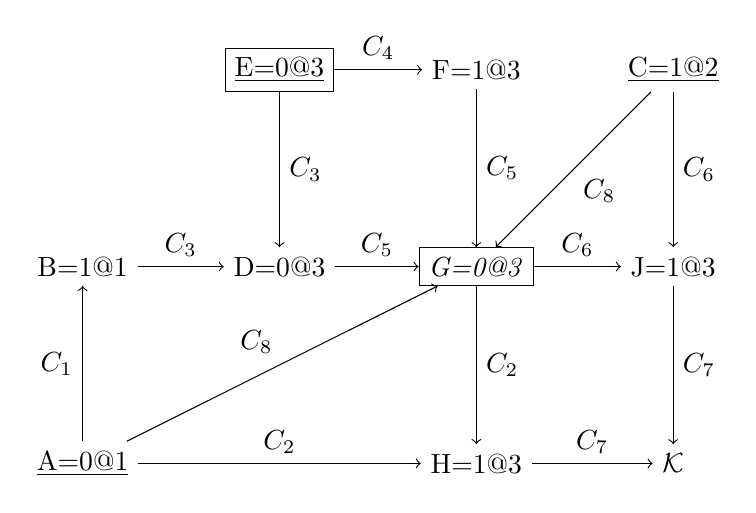
\begin{tikzpicture}[node distance=2.5cm,auto]
	\node (B) {B=1@1};
	\node (A)[below of=B] {\underline{A=0@1}};
	\node (D) [right of=B] {D=0@3};
	\node (G) [right of=D, rectangle, draw=black] {\textit{G=0@3}};
	\node (H) [below of=G] {H=1@3};
	\node (K) [right of=H] {$\mathcal K$};
	\node (E) [above of=D, rectangle, draw=black] {\underline{E=0@3}};
	\node (F) [right of=E] {F=1@3};
	\node (J) [right of=G] {J=1@3};
	\node (C) [above of=J] {\underline{C=1@2}};
	\path[->] (G) edge node {$C_6$} (J);
	\path[->] (F) edge node {$C_5$} (G);
	\path[->] (C) edge node {$C_6$} (J);
	\path[->] (J) edge node {$C_7$} (K);
	\path[->] (E) edge node {$C_3$} (D);
	\path[->] (E) edge node {$C_4$} (F);

	\path[->] (A) edge node {$C_1$} (B);
	\path[->] (B) edge node {$C_3$} (D);
	\path[->] (D) edge node {$C_5$} (G);
	\path[->] (G) edge node {$C_2$} (H);
	\path[->] (H) edge node {$C_7$} (K);
	\path[->] (A) edge node {$C_2$} (H);

	\path[->] (C) edge node {$C_8$} (G);
	\path[->] (A) edge node {$C_8$} (G);
	\end{tikzpicture}
	\label{pic:new_impl_graph}
	\caption{{\protect\small New implication graph with UIPs (nodes with
	rectangles) and the learned clause $c_{8}$.}}
	\end{figure}

	The learned clause $c_{8}$ implies that the node $G$ must be set to $1@3$,
	else $c_{8}$ would be unsatisfied and we get again a new conflict. This
	implies in turn, that the value either in $D$ or in $F$ can be arbitrarily
	chosen. This is also the case for node $J$ and node $H$. One of both nodes
	the value can be arbitrarily chosen and the ohter must be set to $0@3$. By
	setting $F=H=0@3$, we observe that all clauses $c_{i}$, $i\in \{1,\ldots
	,8\} $ are satisfied and obtain a model $M=\{\lnot A,B,C,D,E,F,G,\lnot H,J\}$%
	.

	% \begin{tikzpicture}[node distance=2.5cm,auto]
	% \node (A) {A=0@1};
	% \node (B) [right of=A] {B=1@1};
	% \node (C) [right of=B] {C=1@2};
	% \node (E) [right of=C] {E=1@3};				
	% \path[->] (A) edge node {$c_1$} (B);
	% \end{tikzpicture}
	% \newline
	% \newline
	% The remaining clauses $c_2$, $c_5$, $c_6$ and $c_7$ doesn't contain any
	% rules for the implication graph, so we have to introduce a new decision
	% level $DL 4$ and we can choose the decision for e. g. $G$ as $G = 1@4$:%
	% \newline
	% \bigskip

	% \begin{tikzpicture}[node distance=2.5cm,auto]
	% \node (A) {A=0@1};
	% \node (B) [right of=A] {B=1@1};
	% \node (C) [right of=B] {C=1@2};
	% \node (E) [right of=C] {E=1@3};	
	% \node (G) [right of=E] {G=1@4};			
	% \path[->] (A) edge node {$c_1$} (B);
	% \end{tikzpicture}
	% \newline
	% \newline
	% Again, the remaining clauses $c_5$ and $c_7$ doesn't contain any rules for
	% the implication graph, so we have to introduce a new decision level two
	% times ($DL 5$ and $DL 6$) and we can choose the decisions for e. g. $D$ as $%
	% D = 1@5$ and $H$ as $H = 0@6$:\newline
	% \bigskip

	% \begin{tikzpicture}[node distance=2.5cm,auto]
	% \node (A) {A=0@1};
	% \node (B) [right of=A] {B=1@1};
	% \node (C) [right of=B] {C=1@2};
	% \node (E) [right of=C] {E=1@3};	
	% \node (G) [right of=E] {G=1@4};	
	% \node (D) [below right of=A] {D=1@5};
	% \node (H) [below right of=C] {H=0@6};		
	% \path[->] (A) edge node {$c_1$} (B);
	% \end{tikzpicture}
	% \newline

	% Now we have fulfilled all clauses $c_{i}$, $i\in \{1,...,9\}$ and therefore
	% we can choose any dedcisions for the ramaining values.\newline
	% A valid solution model would be: $\{\lnot A,B,C,D,E,F,G,\lnot H,J\}$

	\bigskip
}

%\solution{
$[p]\sigma = [x:=x+y; \text{ if } x<0 \text{ then } abort \text{ else } while \text{ } x \neq y \text{ } do \text{ }... \text{ } od]\sigma 
\hspace{0.6 cm} \sigma: x \mapsto 1, y \mapsto 1\\
= [\text{if } x<0 \text{ then } abort \text{ else } while \text{ } x \neq y \text{ } do \text{ }... \text{ } od][x:=x+y]\sigma_1
\hspace{1 cm} \sigma_1: x \mapsto [x+y]\sigma = 2\\
\text{} \hspace{12 cm} y \mapsto 1\\
= [\text{if } x<0 \text{ then } abort \text{ else } while \text{ } x \neq y \text{ } do \text{ }... \text{ } od]\sigma_1
\hspace{4 cm} \underbrace{[x<0]\sigma_1=0}_{false}\\
= [\text{while } x \neq y \text{ do } x:=x+1; y:=y+2 \text{ od}]\sigma_1
\hspace{5 cm} \underbrace{[x \neq y]\sigma_1=0}_{true}\\
= [\text{while } x \neq y \text{ do } ... \text{ od}] [x:=x+1;y=y+2]\sigma_1\\
= [\text{while } x \neq y \text{ do } ... \text{ od}] [y:=y+1] [x:=x+1]\sigma_1
\hspace{3 cm} \sigma_2: x \mapsto [x+1]\sigma_1=3\\
\text{} \hspace{11.8 cm} y \mapsto 1\\
= [\text{while } x \neq y \text{ do } ... \text{ od}] [y:=y+2]\sigma_2
\hspace{4.7 cm} \sigma_3: y \mapsto [y+2]\sigma_2=3\\
\text{} \hspace{11.8 cm} x \mapsto 3\\
= [\text{while } x \neq y \text{ do } ... \text{ od}]\sigma_3
\hspace{8 cm} \underbrace{[x \neq y]\sigma_3=0}_{false}\\
= \sigma_3$
%}

\begin{exercise}{1}\label{ex:ifabort}
  Let $p$ be the following program:
  \begin{center}
  \begin{ALG}
    \ASS x{x+y};\\
    \IF\ $x<0$ \THEN\\
    \>\ABORT\\
    \ELSE\\
    \>\WHILE\ $x\neq y$ \DO\\
    \>\>\ASS x{x+1};\\
    \>\>\ASS y{y+2}\\
    \>\OD\\
    \FI
  \end{ALG}
  \end{center}
  Show that $\CA{x=2y\land y>2}p{x=y}$ is totally correct by computing the
  weakest precondition of the program.
\end{exercise}

\subsection{solution}

test



\begin{exercise}{1}
  Let $p$ be the program given in exercise~\ref{ex:ifabort}.
  Use the Hoare calculus to show that
  \[\CA{x=2y\land y>2}p{x=y}\]
  is totally correct.
\end{exercise}

\subsection{solution}

test


\begin{exercise}{1}
  Extend our toy language by statements of the form ``$\kw{assert}\
  e$''. When the condition~$e$ evaluates to true, the program
  continues, otherwise the program aborts.

  Specify the syntax and semantics of the extended language.
  Determine the weakest precondition, the weakest liberal
  precondition, the strongest postcondition, and Hoare rules
  (partial and total correctness) for \kw{assert}-statements.
  Show that they are correct.

  Treat the \kw{assert}-statement as a first-class citizen, i.e., do
  not refer to other program statements in the final result.  However,
  you may use other statements as intermediate steps when deriving the
  rules.
\end{exercise}

\subsection{solution}
The NP-hardness of the \textsc{Frequency-Assignment} problem can be shown by
a reduction to $k$\textsc{-Colorability}, since $k$\textsc{-Colorability} is
in NP.

\noindent At first we have to check \ if \textsc{Frequency-Assignment} id a membership
of NP.

\noindent This can be done by a guess \& check procedure:

\subsubsection{definition}
Let\ $G_{F}=(T,E)$ be an arbitrary undirected graph for \textsc{%
Frequency-Assignment} with $T=\{t_{1},t_{2},\ldots ,t_{n}\}$ and $E^{\prime
}=\{(t_{i},t_{j})\mid t_{i},t_{j}\in T(G_{F})$ with $i\neq j$ s.t. $t_{i}$
and $t_{j}$ are interfering each other$\}\subseteq E=$.$\{(t_{i},t_{j})\mid
t_{i},t_{j}\in T(G_{F})$ with $i\neq j\}$. Let $F=\{f_{1},\ldots ,f_{k}\}$
be an arbitrary set of frequencies and $fr:T(G_{F})\rightarrow F$ a function
for assigning each transmitter-vertex $t\in T(G_{F})$ to a frequency $f\in F$%
.

Guess an arbitrary set of frequencies $F=\{f_{1},\ldots ,f_{k}\}$ of size $k$%
. Then for each transmitter-vertex $t\in T(G_{F})$, verify that $t$ has no
adjacent verteices $u\in T(G_{F})$ with the same frequency $f\in F$, i.e. $%
\forall t_{i},t_{j}\in T(G_{F})$ with $i\neq j$, s.t. $(t_{i},t_{j})\in E$
and $fr(t_{i})\neq fr(t_{j})$. The verification of the edges in $G_{F}$
takes polynomial time in the size of $k=|F|$ and the number of edges $n=|E|$
in $G_{F}$.

It remains to show that \textsc{Frequency-Assignment} is NP-hard, by
reducing \textsc{Frequency-Assignment} to $k$\textsc{-Colorability}.

Let\ $G_{F}=(T,E)$ be an arbitrary undirected graph for \textsc{%
Frequency-Assignment} (as defined above). To prove the correctness of the
reduction, we have to show that following equation holds:%
\begin{equation*}
(G_{F},k)\text{ is a positive instance of \textsc{Frequency-Assignment}}%
\quad \Leftrightarrow \quad (G_{C},k^{\prime })\text{ is a positive instance
of }k\text{\textsc{-Colorability}.}
\end{equation*}

\textbf{Proof:}

\noindent Given an arbitrary instance $(G_{F},k)$ of \textsc{Frequency-Assignment}.
Then an instance of $(G_{C},k^{\prime })$ of $k$\textsc{-Colorability} can
be produced iff, $k=k^{\prime }$ and there exists a function $%
c:V(G_{C})\rightarrow C$, where $C=\{1,\ldots ,k^{\prime }\}$ is a set of
colors of size $k^{\prime }$.

$\Rightarrow :$ Suppose $(G_{F},k)$ is a positive instance of \textsc{%
Frequency-Assignment}. Then $\forall t_{i},t_{j}\in T(G_{F})$ with $i\neq j$%
, every edge $(t_{i},t_{j})\in E(G_{F})$, has pairwise different frequencies
such that $fr(t_{i})\neq fr(t_{j})$. We have to define an assignment
function $\mu $ such that $\mu :fr(t)\rightarrow c(v)$, for all $t\in
T(G_{F})$ and for\ all $v\in V(G_{C})$. Since $(G_{F},k)$ is a positive
instance of \textsc{Frequency-Assignment}, then there exists a corresponding
mapping $\mu $ from each node $t\in T(G_{F})$ to each node $v\in V(G_{C})$,
such that $\forall (t_{i},t_{j})\in E(G_{F}):fr(t_{i})\neq fr(t_{j})$ and 

$\forall (v_{i},v_{j})\in E(G_{C}):c(v_{i})\neq c(v_{j})$ and $i\neq j$ and $%
k=k^{\prime }$. This means that both functions are behaving identical on
each graph, such that $fr=c$, i.e. there is a \textit{bijection} between the
vertex sets of $G_{F}$ and $G_{C}$. Thus, both undirected graphs $G_{F}$ and 
$G_{C}$ are \textit{isomorph}. Hence, $(G_{C},k^{\prime })$ is a positive
instance of $k$\textsc{-Colorability}$.$

$\Leftarrow :$ Suppose that $(G_{C},k^{\prime })$ is a positive instance of $%
k$\textsc{-Colorability}. Then there exists an assignment function $\mu $
(similar as above but in the other direction), such that $\mu
:c(v)\rightarrow fr(t)$ for all $v\in V(G_{C})$ and for all $t\in T(G_{F})$.
Since there exists a bijection on both vertex sets of the graphs $G_{C}$ and 
$G_{F}$, i.e. both graphs are \textit{isomorph}, $(G_{F},k)$ is also a
positive instance of \textsc{Frequency-Assignment}.

\bigskip 


\begin{exercise}{1}
  Verify that the following program doubles the value of~$x$.
  For which inputs does it terminate? Choose appropriate pre-
  and postconditions and show that the assertion is totally correct.
  Use $y=2x_0+x$ as a starting point for the invariant,
  where $x_0$ denotes the initial value of~$x$.
\begin{center}
  \begin{ALG}
    \ASS y{3x};\\
    \WHILE\ $2x\neq y$\ \DO\\
    \>\ASS x{x+1};\\
    \>\ASS y{y+1};\\
    \OD
  \end{ALG}
\end{center}    
\end{exercise}

\subsection{solution}

By trying to prove that $\vDash$ is \textit{co-NP-complete} we whave to show that
\begin{itemize}
 \item entailment is in \textit{co-NP} \dots Membership (through reduction) and
 \item NP-hardness \dots co-NP-complete Problem can be reduced to \textit{entailment}
\end{itemize}

\subsubsection{Membership}
And the counterprove for us that we have to show is that:
$\alpha \vDash \beta \iff \alpha \wedge \neg\beta$ isn't satisfiable.

\noindent We try to show membership through a reduction from \textit{entailment} the well known 
co-NP-complete problem: \textit{co-SAT}.\newline

\noindent Proof $\Rightarrow$:\\
We take a look at \textbf{every truth assignments} for \textit{entailment} what means 
that $\alpha \wedge \neg\beta$ isn't satisfied and therefore \textbf{also true}. \\
The last case - a \textbf{false} \textit{entailment} ($\alpha = true$ and $\beta = false$) 
followes a satisfied $\alpha \wedge \neg\beta$ which is \textbf{also false}.

\noindent Proof $\Leftarrow$:\\
if $\alpha \wedge \neg\beta$ isn't satisfiable the entailment is true.\\
So in case $\alpha \wedge \neg\beta$ is true ($\alpha = true$ and $\beta = false$)
the entailment is not valid too.

\subsubsection{NP-hardness}
We try to show a reduction from \textit{co-SAT} to \textit{entailment}\\

$\alpha \wedge \neg\beta$ isn't satisfiable $\iff \alpha \vDash \beta$\\
And fortunately we already proved this reduction while showing Membership above.\\

\noindent What show's us that \textit{entailment} is NP-hard and complete.

\begin{exercise}{1}
    Show that the following correctness assertion is totally correct.
    Describe the function computed by the program if we consider $a$
    as its input and $c$ as its output.
\begin{center}
  \begin{ALG}
    \ASSERTN1{a\geq0}\\
    \ASS b1;\\
    \ASS c0;\\
    \ASSERTN\INV{b=(c+1)^3\land 0\leq c^3\leq a}\\
    \WHILE\ $b\leq a$\ \DO\\
    \>\ASS d{3*c+6};\\
    \>\ASS c{c+1};\\
    \>\ASS b{b+c*d+1}\\
    \OD\\
    \ASSERTN2{c^3\leq a<(c+1)^3}
  \end{ALG}
\end{center}    
\end{exercise}

\subsection{solution}

\subsubsection{Algorithm}
\begin{algorithm}[h]
\small
\caption{DFS}

\begin{algorithmic}
    \FOR{each vertex $u \in V[G]$}
       \STATE color[u] $\gets$ k
       \STATE $\pi[u] \gets NULL$
    \ENDFOR
    \STATE $time \gets 0$
\end{algorithmic}
\end{algorithm}
% 
% \smallskip
% 
% \begin{algorithmic}
% \Function{DFS-Visit}{$u$}
%     \State color[u] $\gets$ k
%     \State d[u] $\gets$ time $\gets$ time + 1
%     \For {each $v \in Adj[u]$}
%       \State $\triangleright$ explore edge $(u,v)$
%       \If {color[v] = k}
%           \State $\pi[v] \gets u$
%           \State DFS-Visit($v$)
%       %\EndIf
%     %\EndFor
%     \State color[v] $\gets$  k
%     \State f[u] $\gets$ time $\gets$ time + 1
% \EndFunction
% \end{algorithmic}


\subsubsection{Description}
The definition of the tree saies that:
\begin{itemize}
 \item there are no cycles allowed
 \item paths are connected
\end{itemize}


\begin{exercise}{1}
  Prove that the rule
\[
\begin{array}{c}
\WH{\CA{\INV}{\WHILE\ e\ \DO\ p\ \OD}{\INV\land\lnot e}}%
   {\CA{\INV\land e}{p}{\INV}}
\end{array}
\]
is correct regarding partial correctness, i.e., show that
$\CA{\INV}{\WHILE\ e\ \DO\ p\ \OD}{\INV\land\lnot e}$ is partially correct
whenever $\CA{\INV\land e}{p}{\INV}$ is partially correct.
\end{exercise}

\subsection{solution}

test



\begin{exercise}{2}
  Determine the weakest liberal precondition of \WHILE-loops, i.e.,
  find a formula equivalent to $\WLP(\WHILE\ e\ \DO\ p\ \OD, G)$
  similar to the weakest precondition in the course.

  Use your formula to compute the weakest liberal precondition of
  the program 
  \begin{center}
     \ASS z0;
     \WHILE\ $y\neq0$ \DO
       \ASS z{z+x};
       \ASS y{y-1}
     \OD
  \end{center}
  with respect to the postcondition $z=x*y_0$. Compare the result
  to the weakest precondition computed in the course and explain
  the differences.
\end{exercise}

\begin{solution}

test

\end{solution}

\end{document}
